\section{Mechanical Design}\label{sec:pros_mech_design}
\begin{marginfigure}[1.25in]
    \centering
    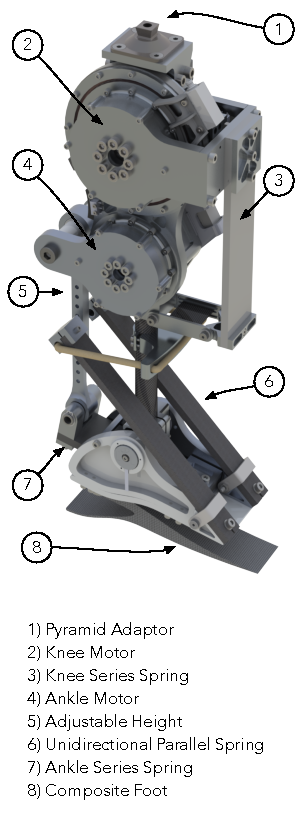
\includegraphics[width=\linewidth]{prosthesis_render_annotated}
    \caption{Render of proposed powered knee and ankle prosthesis design. The
    prosthesis includes series elastic actuators to enable accurate torque
    control and a unidirectional parallel ankle spring to offset the required
    angle torque.}\label{fig:prosthesis_render_annotated}
\end{marginfigure}

\newthought{To test our proposed Neuromuscular control approach}, and its
ability to help subjects maintain or recover their balance, we build a custom
transfemoral prosthesis capable of reproducing dynamic locomotion tasks. The
proposed design, shown in \cref{fig:prosthesis_render_annotated}, uses brushless
electric motors coupled to harmonic drive gear sets to drive both the knee and
ankle joints.  Additionally, the joints employ series elastic actuation to
enable accurate torque control and to protect the prosthesis' gear sets from
sudden impacts.  The design also features a unidirectional parallel spring in
the ankle that partly offsets the torque demands on the ankle motor.  We design
both joints to meet the demands of dynamic locomotion tasks such as running and
trip recovery.

The overall design concept sits in a niche between low powered prostheses
designed with commercial applicability in mind
\citep{sup2007design,sup2009preliminary,lawson2014robotic,rouse2015design,
martinez2011antagonistic} which feature onboard actuation and power sources, and
high-powered tethered systems \citep{caputo2013experimental,
caputo2015informing} with off-board actuation designed exclusively for use in
lab environment. Our design features onboard actuators that are more powerful
than those used in standalone devices, but less capable than those employed in
tethered devices. To ensure a reasonable overall weight the device's batteries,
motor drivers, and computers are off-board. With this design, we expect to be
able to test control ideas without encountering hardware performance limitations
as with a tethered device. At the same time the device is capable of functioning
outside of the lab environment like a standalone prosthesis.

\begin{table*}
    \centering
    \begin{tabular}{lccc}
        \toprule
        Specification         & Desired Value & Theoretical Value
            & Achieved Value\\
        \midrule
        Maximum Knee Torque   & $\unit[160]{N \cdot m}$ 
            & $\unit[170]{N \cdot m}$ & \\
        Maximum Knee Speed    & \unitfrac[1.80]{rev}{s}
            & \unitfrac[1.93]{rev}{sec} & \\
        Knee Torque Bandwidth & \unit[4]{Hz} & \unit[11.7]{Hz} & \\
        Maximum Ankle Torque  & $\unit[200]{N \cdot m}$
            & $\unit[170 \ (+120^*)]{N \cdot m}$ & \\
        Maximum Ankle Speed   & \unitfrac[1.14]{rev}{s} 
            & \unitfrac[1.22]{rev}{s} & \\
        Ankle Torque Bandwidth & \unit[3.5]{Hz} & \unit[5.9]{Hz} & \\
        Weight                & \unit[6.8]{kg} & \unit[5.9]{kg}  & \\
        Minimum Height        & \unit[42.5]{cm} & \unit[42]{cm}  & \\
        \bottomrule
    \end{tabular}
    \vspace{0.25in}
    \caption{Designed and achieved design specifications. ($^*$Maximum total
    ankle torque is $\unit[290]{N \cdot m}$ achieved at \unit[10]{degrees} of
    dorsiflexion.)}\label{tab:pros_requirements}
\end{table*}
\Cref{tab:pros_requirements} shows the desired design specifications for the
transfemoral prosthesis and the values achieved by the final design. To obtain
these design specifications we examined a number of studies that elicited trip
responses.

We specify desired joint torque and speed values to meet the requirements of
demanding tasks such as running. The maximum knee torque specification comes
from the findings of \citet{whitley2008maximum}, who tested the joint torques
used during recovery from a simulated fall. The maximum knee speed requirement
comes from \citet{grabiner1993kinematics}, who tested subjects' responses to
simulated trips induced by unseen obstacles on a walkway. We obtain the maximum
ankle torque requirement from \citet{pijnappels2005early}, who tripped subjects
using a obstacles that could suddenly emerge through the floor. The maximum
ankle speed requirement comes from the running data of
\citet{novacheck1998biomechanics}. We set to the minimum height specification,
measured between the center of the knee and bottom of the foot, to accommodate
the $10^\tn{th}$ percentile female \citep{gordon1988anthropometric}.  Finally,
the required weight corresponds to the mean leg weight of a $50^\tn{th}$
percentile male \citep{winter2009biomechanics}.

\subsection{Knee Joint}
\begin{marginfigure}[2in]
    \centering 
    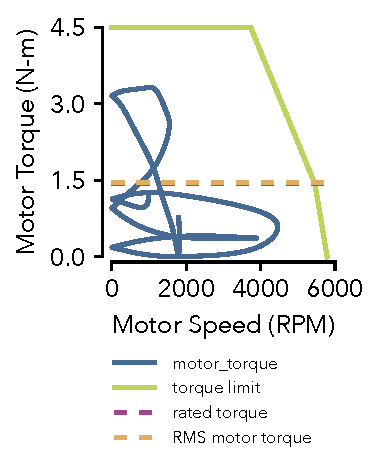
\includegraphics[width=\linewidth]{knee_motor_torque}
    \caption{Knee motor torque required for
    running}\label{fig:knee_motor_torque}
\end{marginfigure}
In addition to achieving the maximum speeds and torques found in
\cref{tab:pros_requirements}, we design the knee joint so that it can reproduce
the torque and speed required for a \unit[80]{kg} person to run at
\unitfrac[3.2]{m}{s} as measured by \citet{novacheck1998biomechanics}. To
reproduce this trajectory in the knee joint, we utilize a RoboDrive ILM
$85\times13$ HS-SP motor coupled to a Harmonic Drive Gear set with a 50:1
reduction (CSG--25--50). \Cref{fig:knee_motor_torque} shows the motor torque
and speed required to reproduce a running trajectory assuming a gear
efficiency of $75\%$. In this plot, we see that the running trajectory lies
within the speed-dependent torque limit of the motor. Moreover, the root mean
squared torque of this trajectory $(\unit[1.46]{N \cdot m})$ exceeds the torque
rating of the motor $(\unit[1.43]{N \cdot m})$ by just $2\%$. Therefore, the
knee joint should be able to provide the necessary torque to enable running for
a short amount of time, or continuously for lighter subjects or at a slightly
reduced speed.

\begin{figure*}[t]
    \centering 
    \includegraphics[width=\linewidth]{knee_design}
    \caption{Internal and external design of the knee 
    joint.}\label{fig:knee_design}
\end{figure*}
\Cref{fig:knee_design} shows the internal and external design of the knee joint.
The primary component in the knee joint is the stator housing. On top of the
housing is a standard pyramid adaptor that allows the prosthesis to connect to
amputee's sockets. Within the stator housing, lies the brushless motor stator,
rotor, and harmonic drive gear set. We sense absolute rotor angle for
commutation of the brushless motor via hall effect sensors and a magnetic
complementary sin/cos encoder. To incorporate series elasticity, we take
inspiration from the design of the bipedal robot Atrias
\citep{grimes2013atrias}, which uses fiberglass series leaf springs. In our
design, the output of the gear set drives the proximal end of a fiberglass leaf
spring in series with the shank. Two Renishaw Resolute absolute encoders measure
the deflection of this spring to enable torque control.

\begin{marginfigure}[2.5in]
    \centering 
    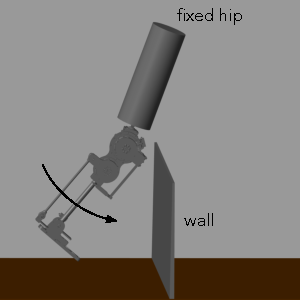
\includegraphics[width=\linewidth]{knee_impact_sim}
    \caption{Impact simulation we used to determine appropriate series spring
    stiffness.}\label{fig:knee_impact_sim}
\end{marginfigure}
In addition to allowing for accurate torque control, as shown by
\citet{au2007biomechanical,au2008powered}, the series elasticity also plays a
crucial role in protecting fragile gear components from impact loads. To choose
the spring stiffness for the knee joint, we simulate the prosthesis impacting a
rigid wall with the foot during swing. To do this, we construct a model of the
prosthesis in Matlab Simulink Simscape Multibody that includes the
series elasticity, gear dynamics, and motor electrical dynamics.
\Cref{fig:knee_impact_sim} shows the simulation environment. The prosthesis is
attached to the distal end of a thigh segment with a fixed hip position. We
control the hip via the ideal swing leg control outlined in
\cref{sec:neuro_ideal_swing} (\cref{eq:hipfeedback}) and consider the case where
the external voltage applied to the motor is zero. This simulation suggests that
a spring stiffness under $\unitfrac[2300]{N \cdot m}{rad}$ will ensure that the
peak impact torque remains lower than the peak allowable impact torque of the
Harmonic Drive of $\unit[242]{N \cdot m}$.

We can also estimate the torque bandwidth of the actuator by analyzing the SEA
dynamics for the system depicted in \cref{fig:sea_diagram}. \todo{check
reference}Assuming the load is fixed, the transfer function between the motor
and load torques is given by
\begin{align}
    \frac{\tau_l}{\tau_m} = \frac{\nicefrac{k}{J_m}}{s^2 + \nicefrac{k}{J_m}}
\end{align}
where $\tau_l$ and $\tau_m$ are the load torque and post-gearbox motor torque
respectively. $J_m$ is the sum of the reflected motor rotor inertia and inertia
of components that form the motor-side attachment of the spring, which has
stiffness $k$. From this equation we calculate the bandwidth of the system
to be
\begin{align}
    f_{3 dB} = \frac{\sqrt{\nicefrac{k}{J_m}}}{2 \pi}.
\end{align}
For a spring stiffness of $\unitfrac[2300]{N \cdot m}{rad}$ we estimate the
torque bandwidth is \unit[11.7]{Hz}. This value exceeds the required torque
bandwidth of \unit[4]{Hz} given by \citet{sergi2012design} (obtained by
analyzing the torque data for walking reported by
\citet{winter2009biomechanics}). However, it should be noted that this is a very
crude estimate of bandwidth. On the one hand, it may underestimate the true
value, as it assumes that to achieve a desired output torque, the motor control
applies the same torque to the motor side of the spring. In practice, a
closed-loop torque control can transiently apply much larger torques to the
motor side in order to achieve faster convergence to a desired steady-state
output torque. On the other hand, this value may also underestimate the true
bandwidth, as it does not consider the motor's voltage-current dynamics or gear
friction.

\subsection{Ankle Joint}
In the ankle joint we utilize a RoboDrive ILM $70\times10$ HS-SP motor coupled
to a Harmonic Drive Gear set with a 100:1 reduction (CSG--20--100). As with the
knee joint, we design the ankle joint to satisfy the requirements listed in
\cref{tab:pros_requirements}. Specifically, for the ankle joint we pay
considerable attention to the tripping condition described by
\citet{pijnappels2005early}, in which the ankle generates a peak torque of
$\unit[202]{N \cdot m}$. 

To avoid using a large and heavy motor to achieve this peak torque, we take
inspiration from previous prosthetic ankle designs that employ a unidirectional
parallel spring in the ankle joint that performs the conservative portion of the
ankle's torque versus angle trajectory during normal walking
\citep{au2007biomechanical,au2008powered,sup2009preliminary,lawson2014robotic}.
The parallel spring offsets the required motor torque, as the actuator only
needs to provide the difference between the desired torque and the torque
provided by the parallel spring. \Cref{fig:ankle_torque_vs_angle_ups} shows the
torque versus angle curve during level ground walking
(\citet{winter2009biomechanics}, scaled to \unit[80]{kg} person). In green we
show the torque generated by a $\unitfrac[700]{N \cdot m}{rad}$ parallel spring
optimized to minimize the root-mean-squared motor torque for this trajectory.
From this plot, we see that with the parallel spring, the peak torque is lower
than the repeated peak torque limit of the Harmonic Drive Gear set.

\begin{marginfigure}[-0in]
    \centering 
    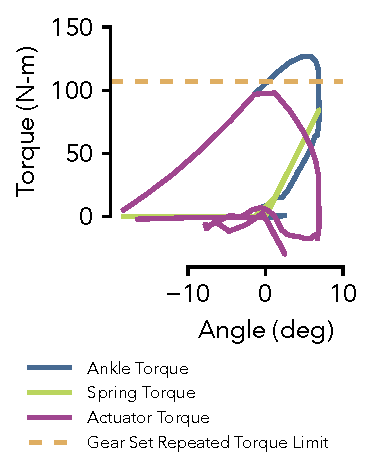
\includegraphics[width=\linewidth]{ankle_torque_vs_angle_ups}
    \caption{Ankle torque vs angle curve during steady, level-ground walking
    (blue) (\citet{winter2009biomechanics} scaled to \unit[80]{kg} person). A
    unidirectional parallel spring can provide a portion of this torque (green)
    and reduces the required actuator torque (purple) to lie under repeated
    torque limit of the Harmonic Drive Gear set (orange).
    }\label{fig:ankle_torque_vs_angle_ups}
\end{marginfigure}

The tripping data obtained by \citet{pijnappels2005early} shows that the ankle
kinematics during trip recovery are similar to those seen during normal walking.
Therefore, the parallel spring, should be able to contribute torque during the
tripping case as well. To confirm this, \cref{fig:ankle_motor_torque_tripping}
shows the motor torque required for trip recovery (obtained by scaling walking
torque data from \citet{winter2009biomechanics} to have a peak torque of
$\unit[202]{N \cdot m})$ We see that the inclusion of the parallel spring allows
the prosthesis to produce enough net torque to reproduce the trip recovery
trajectory without exceeding the torque limit of the motor. 
\begin{figure}[b]
    \centering 
    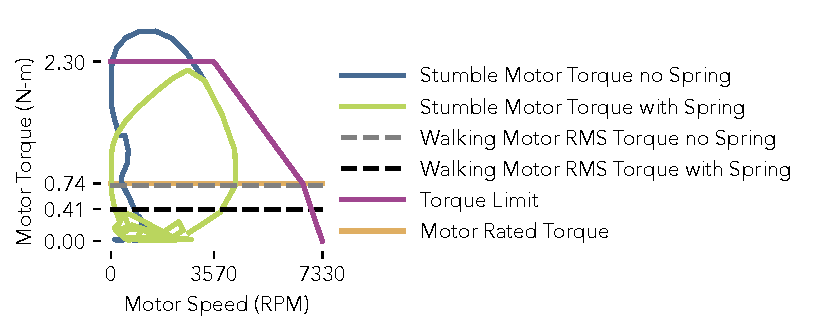
\includegraphics[height=2in]{ankle_motor_torque_tripping}
    \caption{Ankle motor torque required to take the trip recovery action
    observed by \citet{pijnappels2005early} (blue, trajectory obtained by
    scaling walking data from \citet{winter2009biomechanics} to a peak torque of
    $\unit[202]{N \cdot m}$, $75\%$ gear efficiency assumed). Using a parallel
    spring allows the motor to produce the required torque (green) while
    remaining within it's torque limit (purple).
    }\label{fig:ankle_motor_torque_tripping}
\end{figure}

Finally, \cref{fig:ankle_motor_torque_running} shows the torque and speed
required of the motor for running \citep{novacheck1998biomechanics}. In this
case, we use an ankle parallel stiffness of $\unitfrac[267]{N \cdot m}{rad}$.
From this plot, we see that this combination of ankle motor and spring is nearly
sufficient for running. Increasing the voltage of the prosthesis from
\unit[48]{V} to \unit[60]{V} or decreasing the gear ratio from 100:1 to 80:1
will allow the torque trajectory to fit completely within the motor limits. 
\begin{marginfigure}[-0in]
    \centering 
    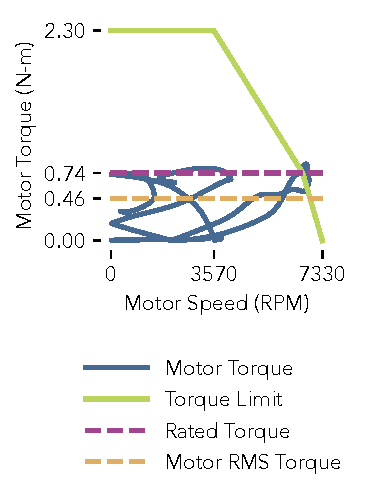
\includegraphics[width=\linewidth]{ankle_motor_torque_running}
    \caption{Ankle motor torque required to reproduce the running trajectory
    recorded by \citet{novacheck1998biomechanics} assuming a parallel spring
    stiffness of $\unitfrac[267]{N \cdot m}{rad}$ and a gear efficiency of
    $75\%$.
    }\label{fig:ankle_motor_torque_running}
\end{marginfigure}

\Cref{fig:ankle_design} shows an internal view of the ankle actuator and
external views of the actuator and foot mechanism. In the ankle design, the
output of the actuator actuates the foot through a four-bar mechanism. The
actuator pulls or pushes on the proximal end of a length-adjustable tendon. The
distal end of the tendon attaches to one end of a fiberglass series elastic leaf
spring that is also connected to the foot. By measuring the angles of the ankle
actuator output and the ankle joint and using the equations of the four-bar
mechanism's kinematics, we can calculate the deflection of the leaf spring and
thus the torque applied to the ankle.
\begin{figure*}[b!]
    \centering 
    \includegraphics[width=\linewidth]{ankle_design}
    \caption{Internal and external design of the ankle 
    joint.}\label{fig:ankle_design}
\end{figure*}

The design of the ankle actuator represents a second iteration of the knee
actuator design and features two main improvements.  First, it has increased
space on the side of the motor for cable routing. Second, the ankle actuator has
a solid rotor shaft. In contrast, the knee actuator's shaft is comprised of two
parts: one that held the motor rotor and transferred power through the gear set,
and another that held the sin/cos encoder's magnetic shaft component. In
practice, these two components proved difficult to align, causing degraded
performance of the sin/cos encoder. The ankle actuator's solid shaft ensures the
encoder magnet stays aligned with the read head.

\begin{marginfigure}[-0.0in]
    \centering 
    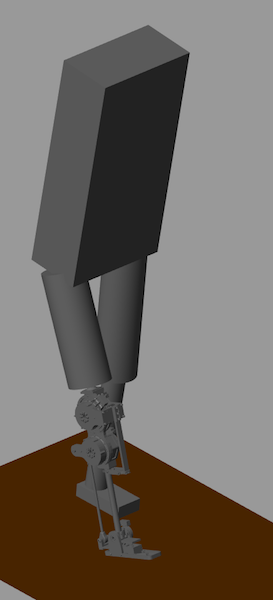
\includegraphics[height=2in]{ankle_impact_sim}
    \caption{Impact simulation we used to determine appropriate series spring
    stiffness.}\label{fig:ankle_impact_sim}
\end{marginfigure}
As we did for the knee series spring, we again determine an acceptable ankle
spring stiffness by performing an impact simulation. For the ankle, we simulate
an \unit[80]{kg} person stepping on the prosthesis when the motor driver
provides the ankle motor with zero applied voltage. \Cref{fig:ankle_impact_sim}
shows the simulation environment. From this simulation we find that a spring
stiffness of about $\unitfrac[1000]{N \cdot m}{rad}$ should sufficiently protect
the ankle gear set from impacts. This estimate is likely softer than necessary
due to the additional series compliance in the amputee's socket and the
composite foot that are not included in the simulation.
Repeating the bandwidth calculation we performed for the knee spring, we
estimate the ankle bandwidth may be around \unit[5.9]{Hz}. This value exceeds
the required torque bandwidth of \unit[3.5]{Hz} given by \citet{au2008powered}
(obtained by analyzing the torque data for walking reported by
\citet{winter2009biomechanics}).
